\chapter{Лабораторная работа 2 \\
Проектирование МШУ с помощью Диаграммы Смита}

Цель работы: научиться работать с шумовыми свойствами линейных устройств, правильно моделировать и проектировать усилительные устройства на минимум коэффициента шума, получить навыки работы со средой моделирования Advanced Design Studio (ADS).

\section{Техническое задание}

Спроектировать малошумящий усилитель на основе биполярного транзистора HBFP0420, работающего на центральной частоте $f_c = 0.7~\text{ГГц}$ и полосой $\Delta f = 30~\text{МГц}$.
В рабочей точке обеспечить $V_{CE} = 2~\text{В}$ и $I_C = 5~\text{мА}$.

\section{Выполнение работы}

Соберём моделируемую схему (Рис.~\ref{fig:low_noise_amplifier_schematic_1}).

Проведём оценку утойчивости в заданном частотном диапазоне (Рис.~\ref{fig:low_noise_amplifier_data_1_sustainability}).

\begin{figure}[!ht]
    \centering
    \begin{subfigure}[b]{0.45\textwidth}
        \centering
        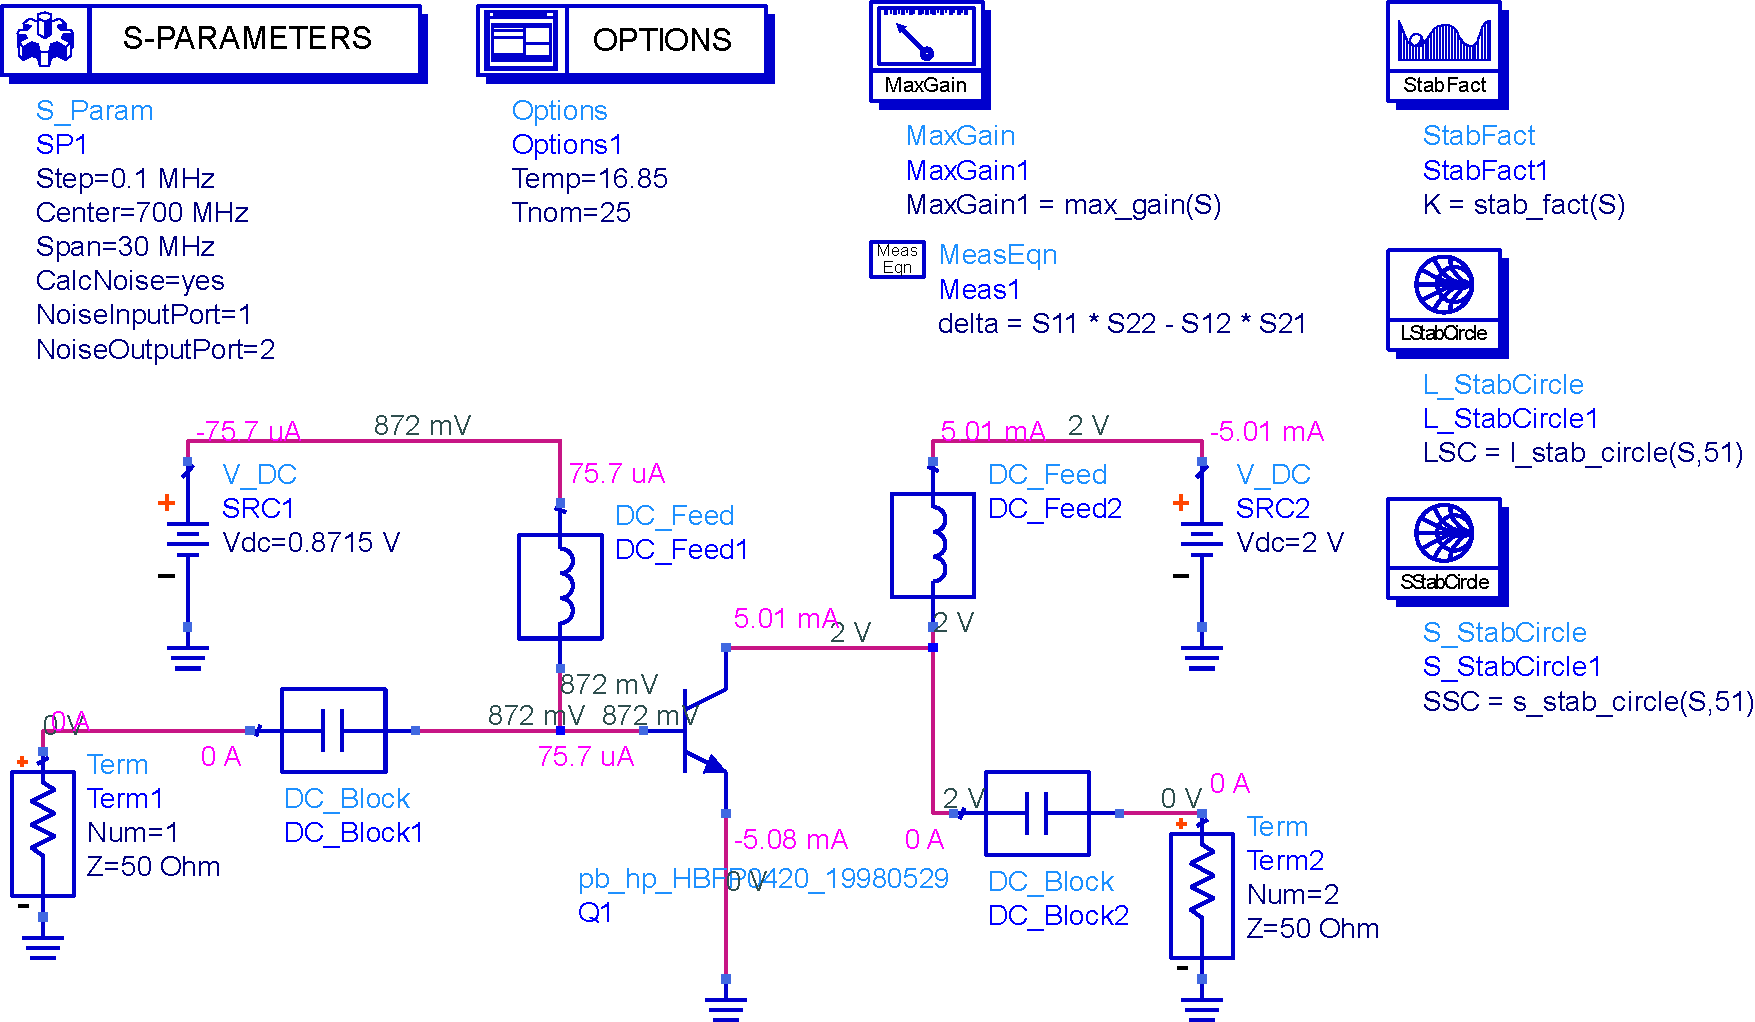
\includegraphics[width=\textwidth]{low_noise_amplifier_schematic_1.pdf}
        \caption{}%
        \label{fig:low_noise_amplifier_schematic_1}
    \end{subfigure}
    \hfill
    \begin{subfigure}[b]{0.45\textwidth}
        \centering
        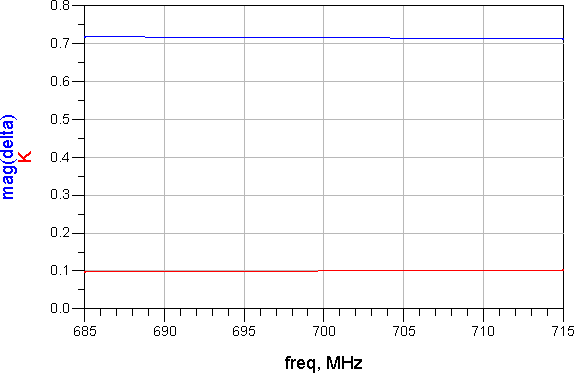
\includegraphics[width=\textwidth]{low_noise_amplifier_data_1_sustainability.pdf}
        \caption{}%
        \label{fig:low_noise_amplifier_data_1_sustainability}
    \end{subfigure}
        \caption{%
            (а) Моделируемая схема;
            (б) оценка устойчивости моделируемой схемы
        }%
        \label{fig:low_noise_amplifier_1}
\end{figure}

Видно, что в рабочем диапазоне $K < 1$, следовательно устройство потенциально неустойчиво.
Спроектируем цепи согласования так, чтоб они не попали в регионы неустойчивости.

\begin{wrapfigure}{r}{0.4\textwidth}
        \centering
        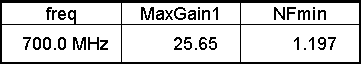
\includegraphics[width=0.4\textwidth]{low_noise_amplifier_data_1_table.pdf}
        \caption{Максимальный коэффициент усиления и минимальный коэффициент шума}%
        \label{fig:low_noise_amplifier_data_1_table}
\end{wrapfigure}
Для продолжения анализа выведем на диаграммы Смита с кругами устойчивойсти входной (Store Sustainability Circle, SSC) и выходной (Load Sustainability Circle, LSC) цепей (Рис.~\ref{fig:low_noise_amplifier_data_1_sustainability_circles}).
Также выведем таблицу с максимально достижимым коэффициентом усиления и минимальным коэффициентом шума (Рис.~\ref{fig:low_noise_amplifier_data_1_table})

\begin{figure}[!ht]
    \centering
    \hfill
    \begin{subfigure}[b]{0.45\textwidth}
        \centering
        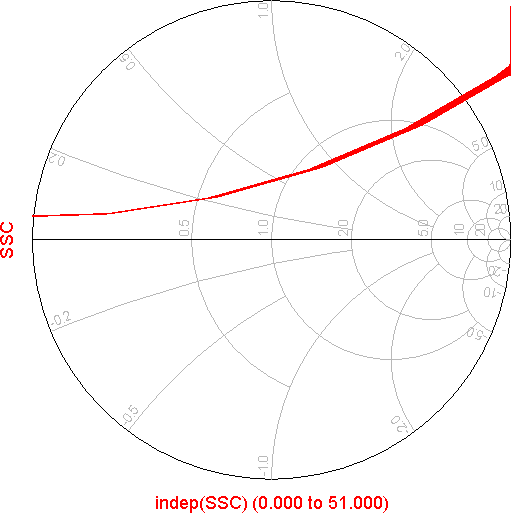
\includegraphics[width=\textwidth]{low_noise_amplifier_data_1_store.pdf}
        \caption{}%
        \label{fig:low_noise_amplifier_data_1_store}
    \end{subfigure}
    \hfill
    \begin{subfigure}[b]{0.45\textwidth}
        \centering
        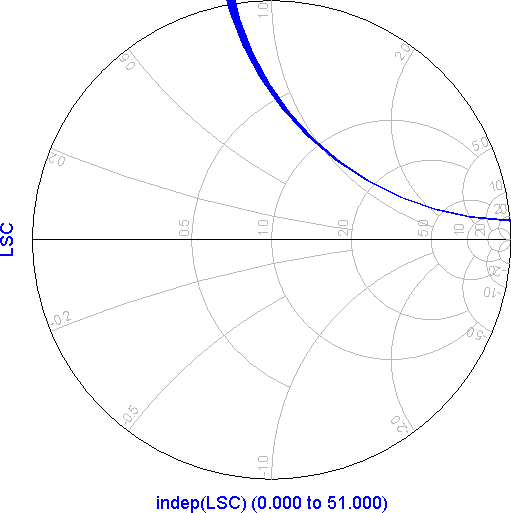
\includegraphics[width=\textwidth]{low_noise_amplifier_data_1_load.pdf}
        \caption{}%
        \label{fig:low_noise_amplifier_data_1_load}
    \end{subfigure}
    \hfill
    \caption{%
        Круги устойчивости:
        (а) входной цепи;
        (б) выходной цепи.
    }%
    \label{fig:low_noise_amplifier_data_1_sustainability_circles}
\end{figure}

Создадим набор кругов постоянного усиления и набор кругов постоянного коэффициента шума (Рис.~\ref{fig:low_noise_amplifier_data_2_equations}) и добавим их на диаграмму Смита (Рис.~\ref{fig:low_noise_amplifier_data_2_store}).
Изменяя добавки в выражениях для \code{gacir\_minus} и \code{nfcir\_plus} подберём такие значения (Рис.~\ref{fig:low_noise_amplifier_data_3_equations}), чтоб эти окружности касались, и точка касания находилась в регионе устойчивости (Рис.~\ref{fig:low_noise_amplifier_data_3_store}).
В случае моделируемой схемы этой точкой будет ($0.371 \angle-15.386$), соответствующая коэффициенту усиления $25.35~\text{дБ}$ и коэффициенту шума $1.297~\text{дБ}$.

\begin{figure}[!ht]
    \centering
    \begin{subfigure}[b]{0.45\textwidth}
        \centering
        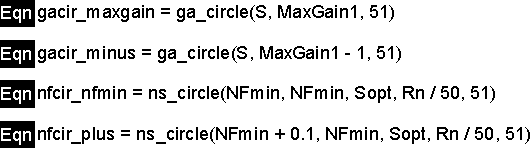
\includegraphics[width=\textwidth]{low_noise_amplifier_data_2_equations.pdf}
        \caption{}%
        \label{fig:low_noise_amplifier_data_2_equations}
    \end{subfigure}
    \hfill
    \begin{subfigure}[b]{0.45\textwidth}
        \centering
        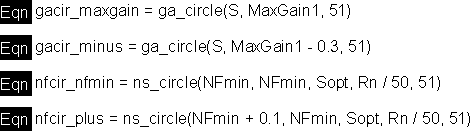
\includegraphics[width=\textwidth]{low_noise_amplifier_data_3_equations.pdf}
        \caption{}%
        \label{fig:low_noise_amplifier_data_3_equations}
    \end{subfigure}
    \vfill
    \begin{subfigure}[b]{0.45\textwidth}
        \centering
        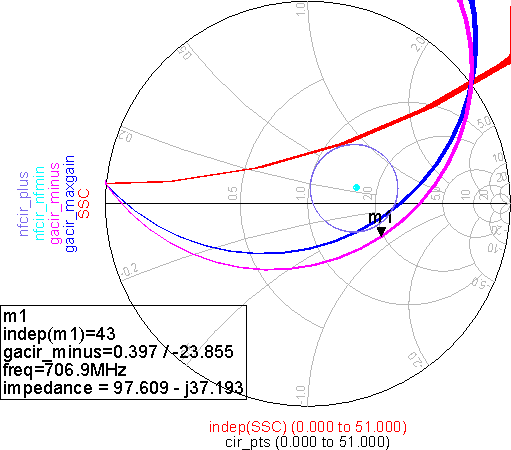
\includegraphics[width=\textwidth]{low_noise_amplifier_data_2_store.pdf}
        \caption{}%
        \label{fig:low_noise_amplifier_data_2_store}
    \end{subfigure}
    \hfill
    \begin{subfigure}[b]{0.45\textwidth}
        \centering
        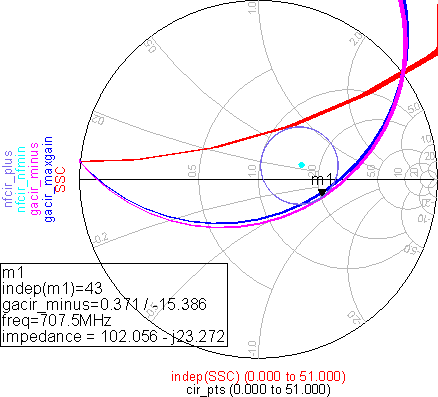
\includegraphics[width=\textwidth]{low_noise_amplifier_data_3_store.pdf}
        \caption{}%
        \label{fig:low_noise_amplifier_data_3_store}
    \end{subfigure}
\end{figure}

Это будет коээфициент отражения входной согласующей цепи со стороны транзистора ($S_{in} = 0.371 \angle -15.386$).

Для определения выходной точки проведём ещё некоторые расчёты (Рис.~\ref{fig:low_noise_amplifier_data_4_equations}). Результаты можно увидеть на рис.~\ref{fig:low_noise_amplifier_data_4_load}.

\begin{figure}[!ht]
    \centering
    \begin{subfigure}[b]{0.55\textwidth}
        \centering
        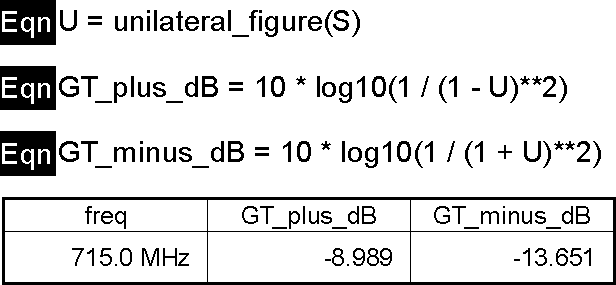
\includegraphics[width=\textwidth]{low_noise_amplifier_data_4_equations.pdf}
        \caption{}%
        \label{fig:low_noise_amplifier_data_4_equations}
    \end{subfigure}
    \hfill
    \begin{subfigure}[b]{0.55\textwidth}
        \centering
        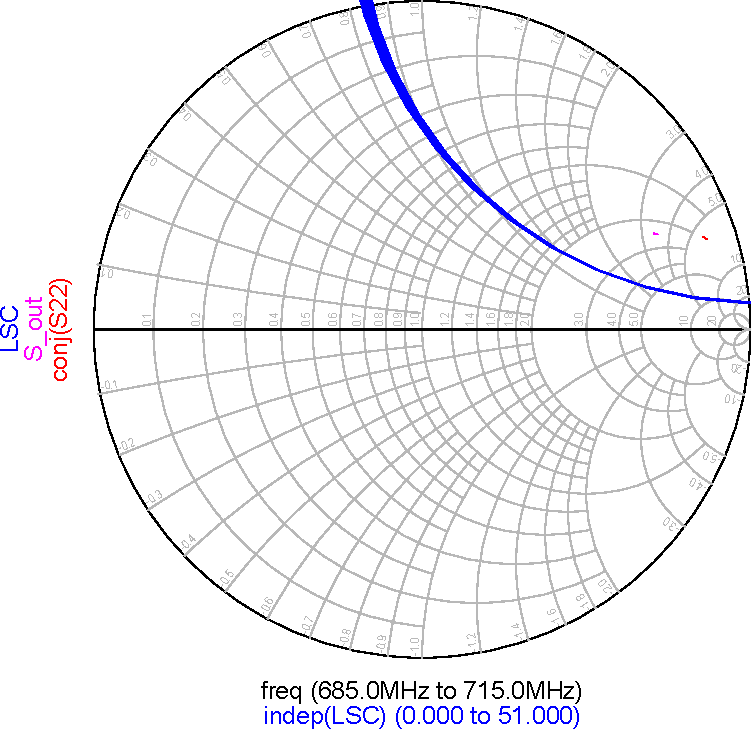
\includegraphics[width=\textwidth]{low_noise_amplifier_data_4_load.pdf}
        \caption{}%
        \label{fig:low_noise_amplifier_data_4_load}
    \end{subfigure}
    \caption{%
        (а) Расчёты для вывода $S_{22}^*$ и $S_{out}$;
        (б) диаграмма Смита
    }%
    \label{fig:low_noise_amplifier_data_4_1}
\end{figure}

Также найдём $S_{out}$ c помощью выражений на рис.~\ref{fig:low_noise_amplifier_data_4_in_out} и выведем его (Рис.~\ref{fig:low_noise_amplifier_data_4_out}).

\begin{figure}[!ht]
    \centering
    \begin{subfigure}[b]{0.7\textwidth}
        \centering
        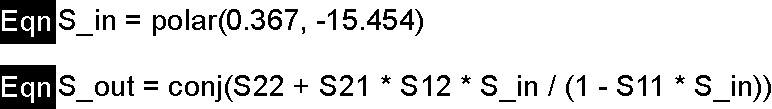
\includegraphics[width=\textwidth]{low_noise_amplifier_data_4_in_out.pdf}
        \caption{}%
        \label{fig:low_noise_amplifier_data_4_in_out}
    \end{subfigure}
    \hfill
    \begin{subfigure}[b]{0.3\textwidth}
        \centering
        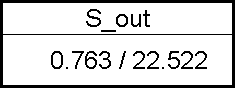
\includegraphics[width=\textwidth]{low_noise_amplifier_data_4_out.pdf}
        \caption{}%
        \label{fig:low_noise_amplifier_data_4_out}
    \end{subfigure}
    \caption{%
        (а) Расчёты для вывода $S_{22}^*$ и $S_{out}$;
        (б) диаграмма Смита
    }%
    \label{fig:low_noise_amplifier_data_4_2}
\end{figure}

Спроектируем согласующие цепи, для чего воспользуемся инструментом \elementname{SmithChart} из палитры \elementname{Smith Chart Matching}.
Соберём схему (Рис.~\ref{fig:low_noise_amplifier_schematic_2}) и поочерёдно сделаем синтез согласующих цепей на входе и выходе транзистора, после чего промоделируем и выведем интересующие нас данные (Рис.~\ref{fig:low_noise_amplifier_data_5_table}).

\begin{figure}[!ht]
    \centering
    \includegraphics[width=0.7\textwidth]{low_noise_amplifier_schematic_2.pdf}
    \caption{Схема с синтезом согласующих цепей}%
    \label{fig:low_noise_amplifier_schematic_2}
\end{figure}

\begin{figure}[!ht]
    \centering
    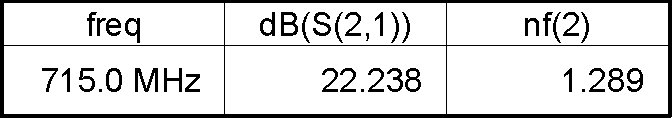
\includegraphics[width=0.4\textwidth]{low_noise_amplifier_data_5_table.pdf}
    \caption{Результаты моделирования}%
    \label{fig:low_noise_amplifier_data_5_table}
\end{figure}
